\documentclass[12pt,a4paper]{report}

\usepackage[utf8]{inputenc}
\usepackage[english]{babel}
\usepackage{amsmath}
\usepackage{amsfonts}
\usepackage{amssymb}
\usepackage{graphicx}
\usepackage{cite}
\usepackage{hyperref}
\usepackage[left=2cm,right=2cm,top=2cm,bottom=2cm]{geometry}

\author{Josep Puig}
\title{Communications Protocols and Network Models}


\begin{document}
\maketitle


\chapter{General Protocols Structure}

\paragraph{}

In addition to hardware compatibility, it is essential that the different parts of a network can understand each other, i.e., software compatibility exists. This is the main reason why a protocol is so important, along with some standards, in case that different parts of the network have been built by different companies and they need to work together. 

Communication Protocol is, in general, a system of rules that allow two or more entities of a communication system to transmit information successfully. The rules can be expressed by algorithms and data structures.

The three main parts of the protocol are the following:

First, the syntax. It means the structure of the presented data. It specifies and separates the group of bits with same meaning.

Second, the semantics. It explains the meaning of each section of bits, which have been defined in the syntax. 

Last, the timing. It specifies the data communication velocity. The sender and the receiver use the same velocity for sending and receiving, so that nor bits are lost (in case the sender sends data faster of what that receiver receives) neither the capacity of reception of the receiver is wasted (in case the sender sends data slower of what the receiver receives).

Referring to standards, there are two main groups:

One, the standards that are so-called “de jure”, which are endorsed by a formal standards organization. They are also known as standards according to law.

And second, the “de facto” standards, which are adopted widely by an industry and its customers. They are also known and market-driven standards. These standards arise when a critical mass like them well enough to collectively use them. 

Some times, market-driven standards can end up being “de jure” standards if they are approved though a formal standard organization. Therefore, a “de facto” standard can become a “de jure” standard.

Specifically talking of space, the main formal standard organization is The Consultative Committee for Space Data Systems. Their recommendations become later part of ISO. In their website, everybody can find their books.



\chapter{Network Models}
A network is composed by both hardware and software, and both parts are essential. The main kind of networks that exist are:
\section{Layered Tasks}
There are different “levels” of the communication. Those levels would be: 
Higher layers: the message is written and encoded following the protocol, if it is the sender, or the message is decoded and read, if it is the receiver. This is done by software.
Middle layers: the message goes from the software to the hardware of sending and gets ready to be sent, if it is the sender, or from the hardware of receiving to the software, if it is the receiver. 
Lower layers: the message is sent, travels along the space, and is received. 
In this network, hierarchy is very important.


\section{The OSI Model}
This network characterizes and standardizes the communication functions without regard to their underlying internal structure and technology. In this model, the communication system are organized into abstraction layers. Those layers are typically physical layer, data link layer, network layer, transport layer, session layer, presentation layer and application layer. 
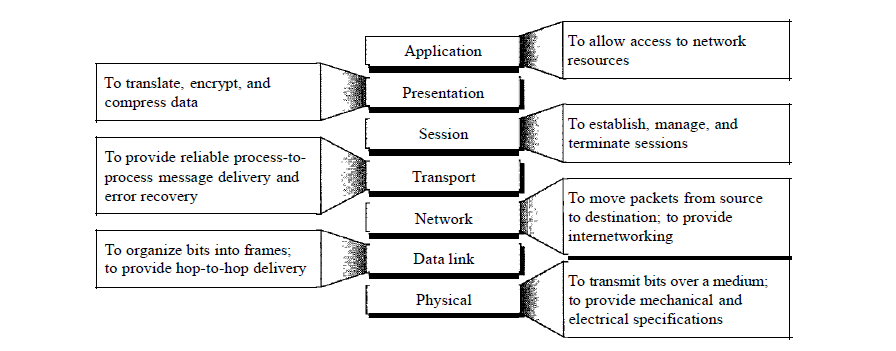
\includegraphics[scale=1]{osi} \newline
\section{TCP/IP Protocol Suite}
This is another computer network model, which is widely used on the Internet and similar computer networks. It stands for Transmission Control Protocol (TCP) and the Internet Protocol (IP). It provides end-to-end data communication specifying how data should be packetized, addressed, transmitted, routed and received. This functionality is organized into four abstraction layers which are used to sort all related protocols according to the scope of networking involved. Those layers are, from lowest to highest, link layer (containing communication methods for data that remains within a single network segment), internal layer (connecting independent networks, providing internetworking), transport layer (handling host-to-host communication), and the application layer (providing process-to-process data exchange for applications). Within the transport layer it is found the segments (TCP/UDP in case of the Internet), within the Network Layer it is found the Packets or Datagrams, and within the link layer there are the frames, such as Wifi, Bluetooth or Ethernet. 


\end{document}
